\chapter{Logical dependencies in key class detection}
\label{cap:usage}

\section{Introduction}
\label{sec:introduction}
Zaidman et al \cite{ZaidmanJurnal} were the first to introduce the concept of key classes and it refers to classes that can be found in documents written to provide an architectural overview of the system or an introduction to the system structure. 
Tahvildari and Kontogiannis have a more detailed definition regarding key classes concept: “Usually, the most important concepts of a system are implemented by very few key classes which can be characterized by the specific properties. These classes, which we refer to as key classes, manage many other classes or use them in order to implement their functionality. The key classes are tightly coupled with other parts of the system. Additionally, they tend to be rather complex, since they implement much of the legacy system’s functionality” \cite{Tahvildari2004ImprovingDQ}.
Also, other researchers use a similar concept as the one defined by Zaidman but under different terms like important classes  \cite{Meyer2014IdentifyingIC} or central software classes \cite{CentralClassesSteidl}.


The key class identification can be done by using different algorithms with different inputs. In the research of Osman et al., the key class identification is made by using a machine learning algorithm and class diagrams as input for the algorithm \cite{6676885}. Thung et al. builds on top of Osman et al.’s approach and adds network metrics and optimistic classification in order to detect key classes \cite{rocclasification}.  

Zaidman et al. use a webmining algorithm and dynamic analysis of the source code to identify the key classes \cite{ZaidmanJurnal}.

Sora et al. use a page ranking algorithm for finding key classes and static analysis of the source code \cite{PagerankENASE}, \cite{enase15}, \cite{SoraSpringer}, \cite{PagerankSACI}. In \cite{Finding-key-classes} the authors use in addition to the previous research also other class attributes to identify important classes.
The page ranking algorithm is a customization of PageRank, the algorithm used to rank web pages \cite{ilprints422}.
The PageRank algorithm works based on a recommendation system. If one node has a connection with another node, then it recommends the second node. In previous works, connections are established based on structural dependencies extracted from static code analysis. If A has a structural dependency with B, then A recommends B, and also B recommends A.

The ranking algorithm ranks all the classes from the source code of the system analyzed according to their importance. To identify the important classes from the rest of the classes a threshold for TOP classes from the top of the ranking is set. The TOP threshold value can go from 1 to the total number of classes found in the system. 

Some researchers \cite{ZaidmanJurnal}, \cite{Ding2016AnIA}, \cite{PAN2018188} consider that 15\% of the total number of classes of the system is a suited value for the TOP threshold. Other researchers \cite{Finding-key-classes} consider that 15\% of the total number of classes is a too high value for the TOP threshold and suggest that a value in the range of 20–30 is better.


\section{Metrics for results evaluation}
\label{sec:evalmetrics}
To evaluate the quality of the key classes ranking algorithm and solution produced, the key classes found by the algorithm are compared with a reference solution.

The reference solution is extracted from the developer documentation.  Classes mentioned in the documentation are considered key classes and form the reference solution (ground truth) used for validation \cite{7551990}. 


For the comparison between both solutions, is used a classification model. The quality of the solution produced is evaluated by using metrics that evaluate the performance of the classification model, such as Precision-Recall and Receiver Operating Characteristic Area Under Curve (ROC-AUC).

A classification model (or "classifier") is a mapping between expected results and predicted results \cite{ROCIntro}, \cite{ROCBRADLEY19971145}. Both results can be labeled as positive or negative, which leads us to the confusion matrix from figure \ref{fig:confusion}. 
\begin{figure}[h]
\centering
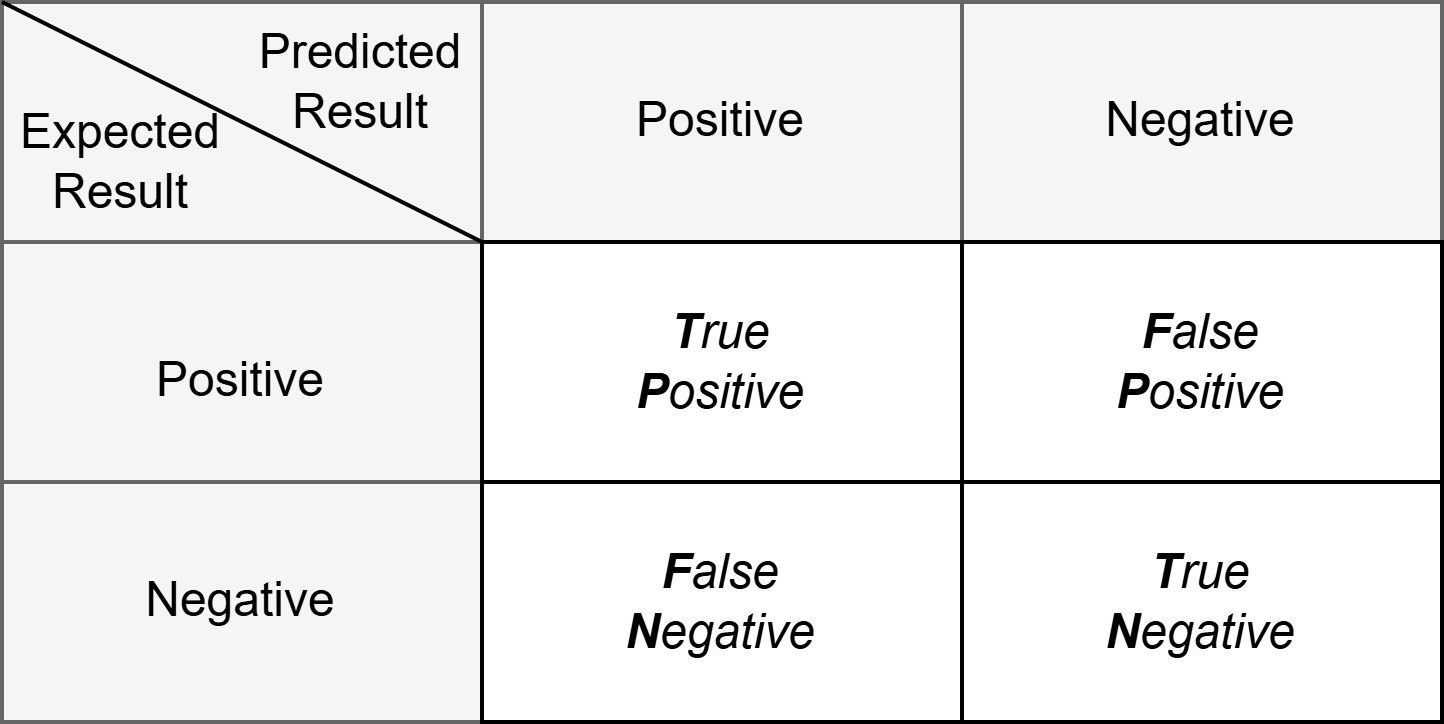
\includegraphics[scale=0.9]{confusion.png}
\caption{Confusion matrix}
\label{fig:confusion}
\centering
\end{figure}
The confusion matrix has the following outcomes:
		\begin{itemize}
			\item \textit{true positive}, if the expected result is positive and the predicted result is also positive.
			\item \textit{false positive}, if the expected result is positive but the predicted result is negative.
			\item \textit{false negative}, if the expected result is negative but the predicted result is positive.
			\item \textit{true negative}, if the expected result is negative and the predicted result is also negative.
		\end{itemize}


\textit{Precision-recall}


Precision is the ratio of True Positives to all the positives of the result set.

\begin{equation}
 precision = \frac{TP}{TP+FN}
\end{equation}
The recall is the ratio of True Positives to all the positives of the reference set.

\begin{equation}
 recall = \frac{TP}{TP+FP}
\end{equation}

As mentioned in section \ref{sec:introduction}, to distinguish the key classes from the rest of the classes a TOP threshold is used. Some researchers consider that 15\% of the total classes is the best value for the TOP threshold and others consider that the value should be in the range of 20-30. 

The precision-recall metric is suited if the threshold value is fixed. If the threshold value is variable, then metrics that capture the behavior over all possible values must be used. Such metric is the Receiver Operating Characteristic metric.

\textit{Receiver Operating Characteristic Area Under Curve}


The ROC graph is a two-dimensional graph that has on the X-axis plotted the false positive rate and on the Y-axis the true positive rate. By plotting the true positive rate and the false positive rate at thresholds that vary between a minimum and a maximum possible value we obtain the ROC curve. The area under the ROC curve is called Area Under the Curve (AUC).

The true positive rate of a classifier is calculated as the division between the number of true positive results identified and all the positive results identified:

\begin{equation}
 True\ positive\ rate (TPR) = \frac{TP}{TP+FN}
\end{equation}
The false positive rate of a classifier is calculated as the division between the number of false positive results identified and all the negative results identified:

\begin{equation}
 False\ positive\ rate (FPR) = \frac{FP}{FP+TN}
\end{equation}


In multiple related works, the ROC-AUC metric has been used to evaluate the results for finding key classes of software systems.
For a classifier to be considered good, its ROC-AUC metric value should be as close to 1 as possible, when the value is 1 then the classifier is considered to be perfect.

Osman et al. obtained in their research an average Area Under the Receiver Operating Characteristic Curve (ROC-AUC) score of 0.750 \cite{6676885}. Thung et al. obtained an average ROC-AUC score of 0.825 \cite{rocclasification}  and Sora et al. obtained an average ROC-AUC score of 0.894 \cite{Finding-key-classes}.


\section{Data set used}
\label{sec:dataset}
In this section, we will look over all the systems studied in the baseline research presented in section \ref{sec:previous_measurements}, and we will try to identify the systems that could be used also in our current research involving logical dependencies.


The research of I. Sora et al \cite{Finding-key-classes} takes into consideration structural public dependencies that are extracted using static analysis techniques and was performed on the object-oriented systems presented in table \ref{tab:keyclass:overview}.

The requirements for a system to qualify as suited for investigations using logical dependencies are: has to be on GitHub, has to have release tags to identify the version, and also has to have an increased number of commits. 
From the total of 14 object-oriented systems listed in the paper \cite{Finding-key-classes}, 13 of them have repositories in Github \ref{tab:gitfoundsystems}. And from the found repositories we identified only 6 repositories that have the same release tag as the specified version from table \ref{tab:keyclass:overview}. It is important to identify the correct release tag for each repository to limit the commits further analyzed by date. Only commits that were made until the specified release are considered and analyzed.
The commits number found on the remaining 6 repositories varies from 19108 commits for Tomcat Catalina to 149 commits for JHotDraw. In order to have more accurate results, we need a significant number of commits, so we reached the conclusion that only 3 systems can be used for key classes detection using logical dependencies: Apache Ant, Hibernate, and Tomcat Catalina.  From all the systems mentioned in table \ref{tab:keyclass:overview} Apache Ant is the most used and analyzed in other  works \cite{enase19}, \cite{7332515}, \cite{1402122}, \cite{Kamran2016IdentificationOC}.

\begin{table}[H]
\renewcommand{\arraystretch}{1}
\caption{Analyzed software systems in previous research paper.}
\label{tab:keyclass:overview}
\centering
\resizebox{\textwidth}{!}{
\begin{tabular}{|c|c|p{7cm}|c|}
\hline
ID	&	System	&	Description	&	Version	\\
\hline
Sl	&	Apache Ant	&	Java library and command line tool that drive the build processes as targets and extension points depending upon each other	&	1.6.1	\\ \hline
S2	&	Argo UML	&	UML modelling tool with support for all UML diagrams.	&	0.9.5	\\ \hline
S3	&	GWT Portlets	&	Open source web framework for building GWT (Google Web Toolkit) Applications.	&	0.9.5 beta	\\ \hline
S4	&	Hibernate 	&	Persistence framework for Java.	&	5.2.12	\\ \hline
S5	&	javaclient	&	Java distributed application for playing with robots	&	2.0.0	\\ \hline
S6	&	jEdit	&	Java mature text editor for programmers.	&	5.1.0	\\ \hline
S7	&	JGAP	&	Genetic Algorithms and Genetic Programming Java library.	&	3.6.3	\\ \hline
S8	&	JHotDraw	&	JHotDraw is a two-dimensional graphics framework for structured drawing editors that is written in Java.	&	6.0b.1	\\ \hline
S9	&	JMeter	&	JMeter is a Java application designed to load test functional behavior and measure performance	&	2.0.1	\\ \hline
S10	&	Log4j	&	Logging Service	&	2.10.0	\\ \hline
S11	&	Mars	&	The Mars Simulation Project is a Java project that models and simulates human settlements on Mars planet	&	3.06.0	\\ \hline
S12	&	Maze	&	The Maze-solver project simulates an artificial intelligence algorithm on a maze	&	1.0.0	\\ \hline
S13	&	Neuroph	&	Neuroph is a Java neural network framework.	&	2.2.0	\\ \hline
S14	&	Tomcat Catalina	&	The Apache Tomcat project is an open-source implementation of JavaServlet and JavaServerPages technologies	&	9.0.4	\\ \hline
S15	&	Wro4J	&	The Wro4J is a web resource (JS and CSS) optimizer for Java.	&	1.6.3	\\ 
\hline
\end{tabular}
}
\end{table}



\begin{table}[H]
\renewcommand{\arraystretch}{1}
\caption{Found systems and versions of the systems in GitHub. }
\label{tab:gitfoundsystems}
\centering
\scalebox{0.8}{
\begin{tabular}{|c|c|c|c|c|}
\hline
ID	&	System	&	Version	&	Release Tag name	&	Commits number	\\
\hline
\rowcolor{lightgreen}
Sl	&	Apache Ant	&	1.6.1	&	rel/1.6.1	&	6713	\\
S2	&	Argo UML	&	0.9.5	&	not found	&	0	\\
S3	&	GWT Portlets	&	0.9.5 beta	&	not found	&	0	\\
\rowcolor{lightgreen}
S4	&	Hibernate 	&	5.2.12	&	5.2.12	&	6733	\\
S5	&	javaclient	&	2.0.0	&	not found	&	0	\\
S6	&	jEdit	&	5.1.0	&	not found	&	0	\\
S7	&	JGAP	&	3.6.3	&	not found	&	0	\\
S8	&	JHotDraw	&	6.0b.1	&	not found	&	149	\\
S9	&	JMeter	&	2.0.1	&	v2\_1\_1	&	2506	\\
S10	&	Log4j	&	2.10.0	&	v1\_2\_10-recalled	&	634	\\
S11	&	Mars	&	3.06.0	&	not found	&	0	\\
S12	&	Maze	&	1.0.0	&	not found	&	0	\\
S13	&	Neuroph	&	2.2.0	&	not found	&	0	\\
\rowcolor{lightgreen}
S14	&	Tomcat Catalina	&	9.0.4	&	9.0.4	&	19108	\\
S15	&	Wro4J	&	1.6.3	&	v1.6.3	&	2871	\\
\hline
\end{tabular}
}
\end{table}



\section{Measurements using logical dependencies}
\label{sec:current_measurements}

As we mentioned in the beginning the purpose is to check if the logical dependencies can improve key class detection. 

As presented in section \ref{sec:previous_measurements}, and section \ref{sec:introduction} the key class detection was done by using structural dependencies of the system. 
In this section, we will use the same tool used in the baseline approach presented in section \ref{sec:previous_measurements}, and we will add a new input to it, the logical dependencies. 

Below is a comparison between the new approach and baseline approach, how we collect the logical dependencies, the results obtained previously, and the new results obtained. 
The new results are separated into two categories, the results obtained by using structural and logical dependencies and the results obtained by using only logical dependencies. 


\subsection{Baseline approach}
\label{sec:previous_measurements}

We use the research of I. Sora et al \cite{Finding-key-classes} as a baseline for our research involving the usage of logical dependencies to find key classes. 
The baseline approach uses a tool that takes as an input the source code of the system and applies ranking strategies to rank the classes according to their importance. 

In order to rank the classes according to their importance, different class metrics are used \cite{Ding2016AnIA}, \cite{ZaidmanJurnal}, \cite{PAN2018188}. Below are presented some of the class metrics used in the baseline approach in order to rank the classes according to their importance.



\subsubsection{Class attributes that characterize key classes}
The metrics used in the baseline research can be grouped into the following categories: 

\begin{itemize}
	\item class size metrics: number of fields (NoF),  number of methods (NoM), global size (Size = NoF+NoM).
	\item class connection metrics, any structural dependency between two classes:
		\begin{itemize}
			\item CONN-IN, the number of distinct classes that use a class;
			\item CONN-OUT, the total number of distinct classes that are used by a class;
			\item CONN-TOTAL, the total number of distinct classes that a class uses or are used by a class (CONN-IN + CONN-OUT).
			\item CONN-IN-W, the total weight of distinct classes that use a class. 
			\item CONN-OUT-W, the total weight of distinct classes that are used by a class. 
			\item CONN-TOTAL-W, the total weight of all connections of the class (CONN-IN-W + CONN-OUT-W) \cite{Finding-key-classes}.
		\end{itemize}
	\item class pagerank values, previous research use pagerank values computed on both directed and undirected, weighted and unweighted graphs:
		\begin{itemize}
			\item PR - value computed on the directed and unweighted graph;
			\item PR-W - value computed on the directed and weighted graph;
			\item PR-U - value computed on the undirected and unweighted graph;
			\item PR-U-W - value computed on the undirected and weighted graph;
			\item PR-U2-W - value computed on the weighted graph with back-recommendations \cite{PagerankENASE}, \cite{enase15}, \cite{Finding-key-classes}, \cite{PagerankSACI}.
		\end{itemize}
\end{itemize}


Based on the class attributes presented, all the classes of the system are ranked. To differentiate the important (key) classes from the rest of the classes, a TOP threshold for the top classes found is set. 
The threshold vary between 20 and 30 classes.



The baseline approach not only identifies the key classes but also evaluates the performance of the solution produced. 
The same approach as the one presented in section \ref{sec:evalmetrics} is used for the evaluation of the results. The key classes found by the ranking algorithm are compared with a reference solution that is extracted from the developer documentation by using a classification model.

The true positives (TP) are the classes found in the reference solution and also in the top TOP ranked classes. False positives (FP) are the classes that are not in the reference solution but are in the TOP ranked classes.
True Negatives (TN) are classes that are found neither in the reference solution nor in the TOP ranked classes. False Negatives (FN) are classes that are found in the reference solution but not found in the TOP ranked classes.


Due to the fact that the TOP threshold is varied, the Receiver Operating Characteristic Area Under Curve metric is used for the evaluation of the results.

The entire workflow of the baseline approach that was presented above is also presented in figure \ref{fig:baseline_approach}.

\begin{figure}[H]
\centering
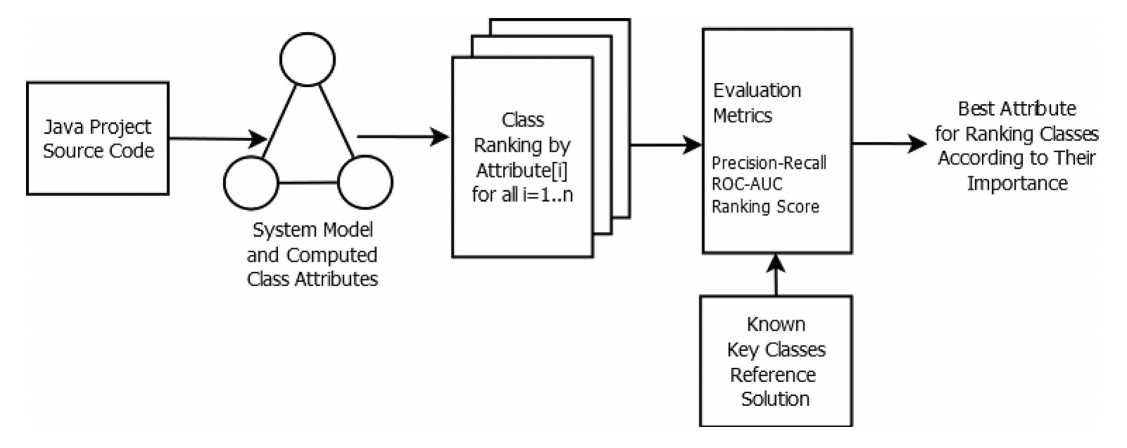
\includegraphics[width=\textwidth]{baseline_approach.PNG}
\caption{Overview of the baseline approach. Reprinted from “Finding key classes in object-oriented
software systems by techniques based on static analysis.” by Ioana Sora and Ciprian-Bogdan Chirila, 2019, Information and Software Technology, 116:106176. Reprinted with permission. }
\label{fig:baseline_approach}
\centering
\end{figure}




\subsection{Comparison with the baseline approach}
\label{sec:comparison}

The baseline approach uses a tool that takes as input the source code of the system to identify the key classes and the reference solution to evaluate the quality of the solution. 
We modified the tool such that it can also take as input the logical dependencies. 

In order to rank the classes according to their importance, the tool uses different class metrics. The list of the metrics used in the baseline approach is presented in section \ref{sec:previous_measurements}.  
The difference in the metrics used compared with the baseline approach is that we use a subset of those metrics. The reason why we are not using all the metrics is that the extracted logical dependencies are undirected. The metrics used by the current approach are CONN-TOTAL, CONN-TOTAL-W, PR-U, PR-U-W, and PR-U2-W.

We did not change the rest of the workflow of the tool. Meaning that the TOP threshold is varied between 20 and 30 and the resulting solution is evaluated by using the ROC-AUC metric. The goal being a ROC-AUC (Receiver Operating Characteristic - Area Under the Curve) metric value as close to 1 as possible.

\begin{figure}[H]
\centering
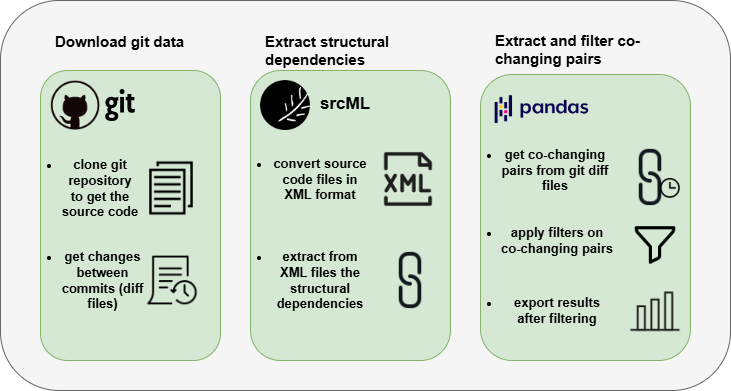
\includegraphics[width=\textwidth]{baseline_comparison.png}
\caption{ Comparison between the new approach and the baseline }
\label{fig:baseline_comparison}
\centering
\end{figure}

\subsection{Logical dependencies collection and current workflow used}

The logical dependencies are those co-changing pairs extracted from the versioning system history that remain after filtering. The filtering part consists of applying two filters: the filter based on commit size and the filter based on connection strength. 

To determine the connection strength of a pair, we first need to calculate the connection factors for both entities that form a co-changing pair.
Assuming that we have a co-changing pair formed by entities A and B, the connection factor of entity A with entity B is the percentage from the total commits involving A that contains entity B. The connection factor of entity B with entity A is the percentage from the total commits involving B that contain also entity A.

\begin{equation}
 connection\ factor\ for\ A = \frac{100 * commits\ involving\ A\ and\ B}{total\ nr\ of\ commits\ involving\ A}
\end{equation}

\begin{equation}
 connection\ factor\ for\ B = \frac{100 * commits\ involving\ A\ and\ B}{total\ nr\ of\ commits\ involving\ B}
\end{equation}

We calculated the connection factor for each entity involved in a co-changing pair and filtered the co-changing pairs based on it. The rule set is that both entities had to have a connection factor with each other greater than the threshold value.

After the filtering part, the remaining co-changing pairs, now called logical dependencies, are exported in CSV files.

The entire process of extracting co-changing pairs from the versioning system, filter them, and export the remaining ones into CSV files is done with a tool written in Python.

The next step is to use the exported logical dependencies for key classes detection. In order to do that we used the same key class detection tool used in the previous research presented in section \ref{sec:previous_measurements}. We adapted the tool to be able to process also logical dependencies because previously the tool used only structural dependencies extracted from the source code of the software systems. 
The workflow is presented in figure \ref{fig:workflow_key}

\begin{figure}[H]
\centering
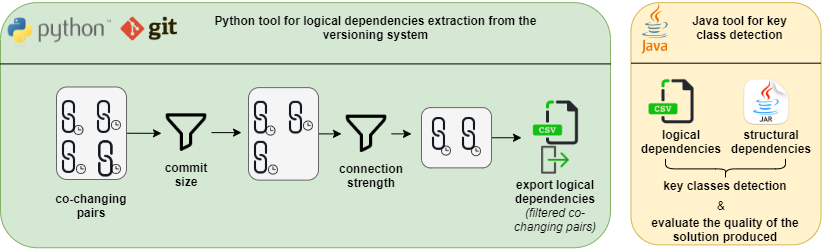
\includegraphics[width=\textwidth]{key_class_workflow.png}
\caption{Workflow for key classes detection}
\label{fig:workflow_key}
\centering
\end{figure}


\subsection{Measurements using only the baseline approach}


In table \ref{tab:previousresults} are presented the ROC-AUC values for different attributes computed for the systems Ant, Tomcat Catalina, and Hibernate by using the baseline approach. We intend to compare these values with the new values obtained by using also logical dependencies in key class detection.

\begin{table}[!h]
\renewcommand{\arraystretch}{1}
\caption{ROC-AUC metric values extracted. }
\label{tab:previousresults}
\centering
\scalebox{0.9}{
\begin{tabular}{|c|ccc|}
\hline
Metrics &	Ant	&	Tomcat Catalina	&	Hibernate	\\
\hline

PR\_U2\_W	&	0.95823	&	0.92341	&	0.95823	\\
PR	&	0.94944	&	0.92670	&	0.94944	\\
PR\_U	&	0.95060	&	0.93220	&	0.95060	\\
CONN\_TOTAL\_W	&	0.94437	&	0.92595	&	0.94437	\\
CONN\_TOTAL	&	0.94630	&	0.93903	&	0.94630	\\

\hline
\end{tabular}
}
\end{table}





\subsection{Measurements using combined structural and logical dependencies}

The tool used in the baseline approach runs a graph-ranking algorithm. 
The graph used contains the structural dependencies extracted from static source code analysis.
Each edge in the graph represents a dependency, the entities that form a structural dependency are represented as vertices in the graph. 
As mentioned in section \ref{sec:comparison}, we modified the tool to read also logical dependencies and add them to the graph. 
In this section, we add in the graph the logical dependencies together with the structural dependencies. 

In tables \ref{tab:measurementscombined:ant}, \ref{tab:measurementscombined:tomcat}, and \ref{tab:measurementscombined:hibernate}, on each line, we have the metric that is calculated and on each column, we have the connection strength threshold that was applied to the logical dependencies used in identifying the key classes.
We started with logical dependencies that have a connection strength greater than 10\%, which means that in at least 10\% of the commits involving A or B, A and B update together. Then we increased the threshold value by 10 until we remained only with entities that update in all the commits together. The last column contains the results obtained previously by the tool by only using structural dependencies.

As for the new results obtained by combining structural and logical dependencies, highlighted with orange are the values that are close to the previously registered values but did not surpass them. Highlighted with green are values that are better than the previously registered values. At this step, we can also observe that for all three systems measured in tables \ref{tab:measurementscombined:ant}, \ref{tab:measurementscombined:tomcat}, and \ref{tab:measurementscombined:hibernate}, the best values obtained are for connection strength between 40-70\%.

\begin{table}[!h]
\renewcommand{\arraystretch}{1}
\caption{Measurements for Ant using structural and logical dependencies combined}
\label{tab:measurementscombined:ant}
\centering
\scalebox{0.7}{
\begin{tabular}{|c|cccccccccc|c|}
\hline
Metrics &	$\geq10\%$	&	$\geq20\%$		&	$\geq30\%$		&	$\geq40\%$		&	$\geq50\%$		&	$\geq60\%$		&	$\geq70\%$		&	$\geq80\%$		&	$\geq90\%$		&	$\geq100\%$		&	Baseline \\
\hline

PR\_U2\_W	&	0.924	&	0.925	&	0.926	&	0.927	&	0.927	&	0.927	&	\cellcolor{lightgreen}0.929	&	0.928	&	0.928	&	0.928	&	0.929	\\
PR	&	0.914	&	0.854	&	0.851	&	\cellcolor{lightgreen}0.866	&	\cellcolor{lightgreen}0.876	&	\cellcolor{lightgreen}0.882	&	\cellcolor{lightgreen}0.887	&	0.854	&	0.852	&	0.852	&	0.855	\\
PR\_U	&	0.910	&	0.930	&	0.933	&	0.933	&	\cellcolor{lightgreen}0.935	&	\cellcolor{lightgreen}0.934	&	\cellcolor{lightgreen}0.939	&	0.933	&	0.933	&	0.933	&	0.933	\\
CON\_T\_W	&	0.924	&	0.928	&	0.931	&	0.932	&	0.933	&	0.934	&	\cellcolor{lightgreen}0.936	&	0.934	&	0.934	&	0.934	&	0.934	\\
CON\_T	&	0.840	&	0.886	&	0.904	&	0.909	&	0.915	&	0.923	&	0.932	&	0.935	&	\cellcolor{lightorange}0.936	&	\cellcolor{lightorange}0.936	&	0.942	\\

\hline
\end{tabular}
}
\end{table}


\begin{table}[!h]
\renewcommand{\arraystretch}{1}
\caption{Measurements for Tomcat using structural and logical dependencies combined}
\label{tab:measurementscombined:tomcat}
\centering
\scalebox{0.7}{
\begin{tabular}{|c|cccccccccc|c|}
\hline
Metrics &	$\geq10\%$	&	$\geq20\%$		&	$\geq30\%$		&	$\geq40\%$		&	$\geq50\%$		&	$\geq60\%$		&	$\geq70\%$		&	$\geq80\%$		&	$\geq90\%$		&	$\geq100\%$		&	Baseline \\
\hline

PR\_U2\_W	&	0.910	&	0.917	&	0.923	&	\cellcolor{lightgreen}0.924	&	\cellcolor{lightgreen}0.924	&	\cellcolor{lightgreen}0.924	&	\cellcolor{lightgreen}0.924	&	\cellcolor{lightgreen}0.924	&	\cellcolor{lightgreen}0.924	&	\cellcolor{lightgreen}0.924	&	0.923	\\
PR	&	0.811	&	0.800	&	0.815	&	0.834	&	0.847	&	0.852	&	0.853	&	0.858	&	0.858	&	0.858	&	0.927	\\
PR\_U	&	0.910	&	0.921	&	0.931	&	\cellcolor{lightgreen}0.933	&	\cellcolor{lightgreen}0.933	&	0.932	&	\cellcolor{lightgreen}0.933	&	0.932	&	0.932	&	0.932	&	0.932	\\
CON\_T\_W	&	0.914	&	0.920	&	0.924	&	\cellcolor{lightorange}0.926	&	0.926	&	0.926	&	0.926	&	0.926	&	0.926	&	0.926	&	0.926	\\
CON\_T	&	0.868	&	0.906	&	0.930	&	0.936	&	0.937	&	\cellcolor{lightorange}0.938	&	0.938	&	0.938	&	0.938	&	0.938	&	0.939	\\
																												

\hline
\end{tabular}
}
\end{table}


\begin{table}[!h]
\renewcommand{\arraystretch}{1}
\caption{Measurements for Hibernate using structural and logical dependencies combined}
\label{tab:measurementscombined:hibernate}
\centering
\scalebox{0.7}{
\begin{tabular}{|c|cccccccccc|c|}
\hline
Metrics &	$\geq10\%$	&	$\geq20\%$		&	$\geq30\%$		&	$\geq40\%$		&	$\geq50\%$		&	$\geq60\%$		&	$\geq70\%$		&	$\geq80\%$		&	$\geq90\%$		&	$\geq100\%$		&	Baseline \\
\hline

PR\_U2\_W	&	0.954	&	0.957	&	\cellcolor{lightorange}0.958	&	0.958	&	0.958	&	0.958	&	0.958	&	0.958	&	0.958	&	0.958	&	0.958	\\
PR	&	0.929	&	0.929	&	0.933	&	0.939	&	0.939	&	0.946	&	\cellcolor{lightorange}0.947	&	0.947	&	0.947	&	0.947	&	0.949	\\
PR\_U	&	0.942	&	0.947	&	0.948	&	0.949	&	0.949	&	\cellcolor{lightorange}0.950	&	0.950	&	0.950	&	0.950	&	0.950	&	0.951	\\
CON\_T\_W	&	0.939	&	0.942	&	0.943	&	0.944	&	0.944	&	\cellcolor{lightgreen}0.945	&	\cellcolor{lightgreen}0.945	&	\cellcolor{lightgreen}0.945	&	\cellcolor{lightgreen}0.945	&	\cellcolor{lightgreen}0.945	&	0.944	\\
CON\_T	&	0.924	&	0.933	&	0.938	&	0.941	&	0.941	&	0.944	&	\cellcolor{lightorange}0.945	&	0.945	&	0.945	&	0.945	&	0.946	\\


\hline
\end{tabular}
}
\end{table}





\subsection{Measurements using only logical dependencies}
In the previous section, we added in the graph based on which the ranking algorithm works the logical and structural dependencies. In the current section, we will add only the logical dependencies to the graph.

In tables \ref{tab:measurementshistory:ant}, \ref{tab:measurementshistory:tomcat}, and \ref{tab:measurementshistory:hibernate}, are presented the results obtained by using only logical dependencies to detect key classes. The measurements obtained are not as good as using logical and structural dependencies combined or using only structural dependencies. But, all the values obtained are above 0.5, which means that a good part of the key classes is detected by only using logical dependencies.  As mentioned in section \ref{sec:evalmetrics}, a classifier is good if it has the ROC-AUC value as close to 1 as possible. 


One possible explanation for the less performing results is that the key classes may have a better design than the rest of the classes, which means that are less prone to change. If the key classes are less prone to change, this implies that the number of dependencies extracted from the versioning system can be less than for other classes.

\begin{table}[!h]
\renewcommand{\arraystretch}{1}
\caption{Measurements for Ant using only logical dependencies}
\label{tab:measurementshistory:ant}
\centering
\scalebox{0.7}{
\begin{tabular}{|c|cccccccccc|c|}
\hline
Metrics &	$\geq10\%$	&	$\geq20\%$		&	$\geq30\%$		&	$\geq40\%$		&	$\geq50\%$		&	$\geq60\%$		&	$\geq70\%$		&	$\geq80\%$		&	$\geq90\%$		&	$\geq100\%$		&	Baseline \\
\hline

PR\_U2\_W	&	0.720	&	0.627	&	0.718	&	0.703	&	0.732	&	0.824	&	0.852	&	\cellcolor{lightorange}0.881	&	0.876	&	0.876	&	0.929	\\
PR	&	0.720	&	0.627	&	0.718	&	0.703	&	0.732	&	0.824	&	0.852	&	\cellcolor{lightorange}0.881	&	0.876	&	0.876	&	0.855	\\
PR\_U	&	0.720	&	0.627	&	0.718	&	0.703	&	0.732	&	0.824	&	0.852	&	\cellcolor{lightorange}0.881	&	0.876	&	0.876	&	0.933	\\
CON\_T\_W	&	0.722	&	0.581	&	0.644	&	0.676	&	0.727	&	0.819	&	0.842	&	0.874	&	\cellcolor{lightorange}0.876	&	0.876	&	0.934	\\
CON\_T	&	0.722	&	0.581	&	0.644	&	0.676	&	0.727	&	0.819	&	0.842	&	0.874	&	\cellcolor{lightorange}0.876	&	0.876	&	0.942	\\

\hline
\end{tabular}
}
\end{table}


\begin{table}[!h]
\renewcommand{\arraystretch}{1}
\caption{Measurements for Tomcat using only logical dependencies}
\label{tab:measurementshistory:tomcat}
\centering
\scalebox{0.7}{
\begin{tabular}{|c|cccccccccc|c|}
\hline
Metrics &	$\geq10\%$	&	$\geq20\%$		&	$\geq30\%$		&	$\geq40\%$		&	$\geq50\%$		&	$\geq60\%$		&	$\geq70\%$		&	$\geq80\%$		&	$\geq90\%$		&	$\geq100\%$		&	Previous \\
\hline

PR\_U2\_W	&	0.672	&	0.656	&	0.645	&	0.697	&	0.754	&	0.776	&	0.786	&	\cellcolor{lightorange}0.799	&	0.799	&	0.799	&	0.923	\\
PR	&	0.685	&	0.643	&	0.642	&	0.697	&	0.754	&	0.776	&	0.786	&	\cellcolor{lightorange}0.799	&	0.799	&	0.799	&	0.927	\\
PR\_U	&	0.685	&	0.643	&	0.644	&	0.697	&	0.754	&	0.776	&	0.786	&	\cellcolor{lightorange}0.799	&	0.799	&	0.799	&	0.932	\\
CON\_T\_W	&	0.694	&	0.636	&	0.636	&	0.697	&	0.754	&	0.776	&	0.786	&	\cellcolor{lightorange}0.799	&	0.799	&	0.799	&	0.926	\\
CON\_T	&	0.654	&	0.611	&	0.636	&	0.697	&	0.754	&	0.776	&	0.786	&	\cellcolor{lightorange}0.799	&	0.799	&	0.799	&	0.939	\\

				
\hline
\end{tabular}
}
\end{table}


\begin{table}[!h]
\renewcommand{\arraystretch}{1}
\caption{Measurements for Hibernate using only logical dependencies}
\label{tab:measurementshistory:hibernate}
\centering
\scalebox{0.7}{
\begin{tabular}{|c|cccccccccc|c|}
\hline
Metrics &	$\geq10\%$	&	$\geq20\%$		&	$\geq30\%$		&	$\geq40\%$		&	$\geq50\%$		&	$\geq60\%$		&	$\geq70\%$		&	$\geq80\%$		&	$\geq90\%$		&	$\geq100\%$		&	Baseline \\
\hline

PR\_U2\_W	&	0.657	&	0.564	&	0.601	&	0.619	&	0.622	&	0.650	&	0.653	&	\cellcolor{lightorange}0.654	&	0.654	&	0.654	&	0.958	\\
PR	&	0.644	&	0.564	&	0.601	&	0.619	&	0.622	&	0.650	&	0.653	&	\cellcolor{lightorange}0.654	&	0.654	&	0.654	&	0.949	\\
PR\_U	&	0.644	&	0.564	&	0.601	&	0.619	&	0.622	&	0.650	&	0.653	&	\cellcolor{lightorange}0.654	&	0.654	&	0.654	&	0.951	\\
CON\_T\_W	&	0.649	&	0.564	&	0.601	&	0.619	&	0.622	&	0.650	&	0.653	&	\cellcolor{lightorange}0.654	&	0.654	&	0.654	&	0.944	\\
CON\_T	&	0.644	&	0.564	&	0.601	&	0.619	&	0.622	&	0.650	&	0.653	&	\cellcolor{lightorange}0.654	&	0.654	&	0.654	&	0.946	\\


\hline
\end{tabular}
}
\end{table}

\section{Correlation between details of the systems and results}
\label{sec:overlapping}

In this section, we discuss about the correlation between the details of the systems and the results obtained in section \ref{sec:current_measurements}.

The reason why we are doing this correlation is to find if there are some links between the details of the systems and the results obtained. 

The results obtained are presented in figures \ref{fig:plot_sd_ld_ant} - \ref{fig:plot_ld_hibernate}. We are using plots to display the results obtained to have a clearer view of how the results fluctuate over different thresholds values.




\begin{figure}[H]
\centering
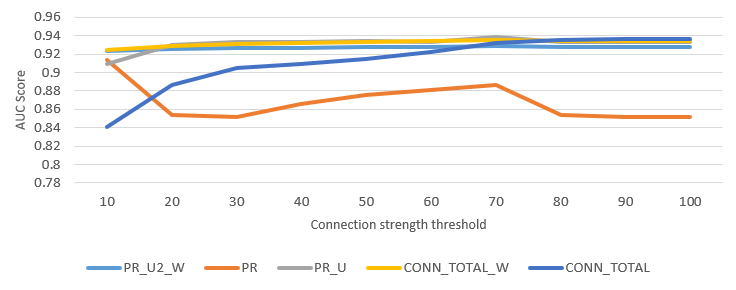
\includegraphics[width=\columnwidth]{ant_SD_LD.PNG}
\caption{Variation of AUC score when varying connection strength threshold for Ant. Results for structural and logical dependencies combined. }
\label{fig:plot_sd_ld_ant}
\centering
\end{figure}


\begin{figure}[H]
\centering
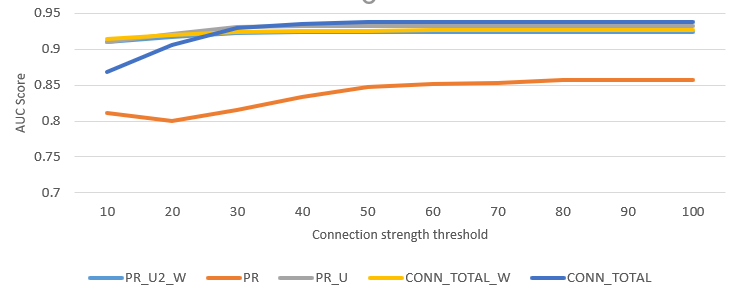
\includegraphics[width=\columnwidth]{tomcat_SD_LD.PNG}
\caption{Variation of AUC score when varying connection strength threshold for Tomcat. Results for structural and logical dependencies combined. }
\label{fig:plot_sd_ld_tomcat}
\centering
\end{figure}


\begin{figure}[H]
\centering
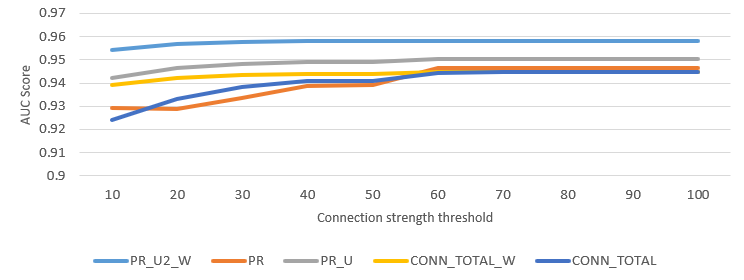
\includegraphics[width=\columnwidth]{hibernate_SD_LD.PNG}
\caption{Variation of AUC score when varying connection strength threshold for Hibernate. Results for structural and logical dependencies combined. }
\label{fig:plot_sd_ld_hibernate}
\centering
\end{figure}



\begin{figure}[H]
\centering
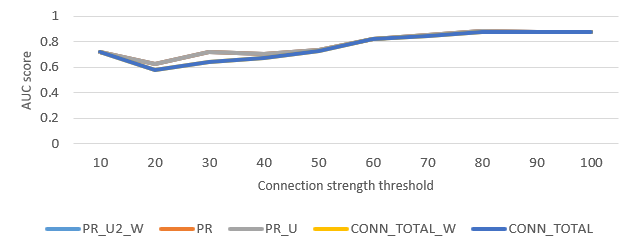
\includegraphics[width=\columnwidth]{ant_LD.PNG}
\caption{Variation of AUC score when varying connection strength threshold for Ant. Results for logical dependencies only. }
\label{fig:plot_ld_ant}
\centering
\end{figure}


\begin{figure}[H]
\centering
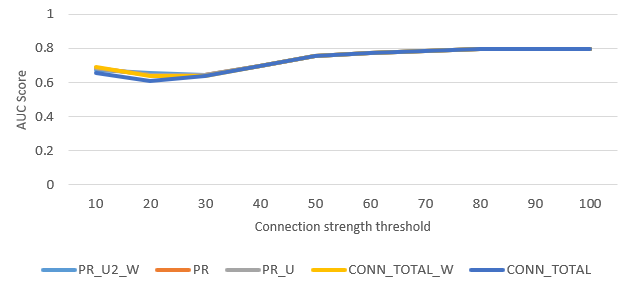
\includegraphics[width=\columnwidth]{tomcat_LD.PNG}
\caption{Variation of AUC score when varying connection strength threshold for Tomcat. Results for logical dependencies only. }
\label{fig:plot_ld_tomcat}
\centering
\end{figure}


\begin{figure}[H]
\centering
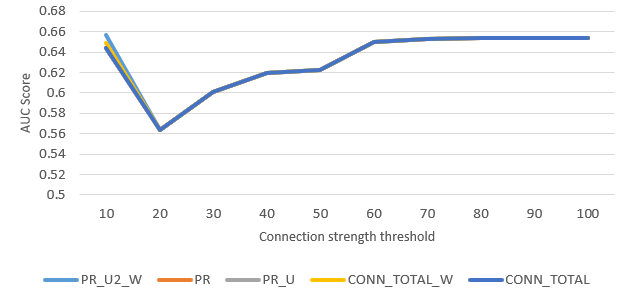
\includegraphics[width=\columnwidth]{hibernate_LD.PNG}
\caption{Variation of AUC score when varying connection strength threshold for Hibernate. Results for logical dependencies only.}
\label{fig:plot_ld_hibernate}
\centering
\end{figure}


The details of the systems are presented in two tables.  In table \ref{tab:overlap} are the overlappings between structural and logical dependencies expressed in percentages. Each column represents the percentage of logical dependencies that are also structural, for each column the logical dependencies are obtained by applying a different connection strength filter. The connection strength filter begins at 10, meaning that in at least 10 \% of the total commits involving two entities, the entities update together. We increase the connection strength filter by 10 up until we reach 100, meaning that in all the commits that involve one entity, the other entity is present also.


In table \ref{tab:ratio_sd_ld} are the ratio numbers between structural dependencies and logical dependencies. We added this table in order to highlight how different the total number of both dependencies is.


\begin{table}[!h]
\renewcommand{\arraystretch}{1}
\caption{Percentage of logical dependencies that are also structural dependencies}
\label{tab:overlap}
\centering
\scalebox{0.7}{
\begin{tabular}{|c|cccccccccc|}
\hline
System &	$\geq10\%$	&	$\geq20\%$		&	$\geq30\%$		&	$\geq40\%$		&	$\geq50\%$		&	$\geq60\%$		&	$\geq70\%$		&	$\geq80\%$		&	$\geq90\%$		&	$\geq100\%$ \\
\hline
Ant	&	25.202	&	34.419	&	36.385	&	34.656	&	33.528	&	33.333	&	28.659	&	33.333	&	35.294	&	35.294	\\
Tomcat Catalina	&	4.059	&	22.089	&	25.000	&	25.758	&	25.926	&	37.525	&	47.368	&	55.285	&	75.000	&	76.923	\\
Hibernate	&	6.546	&	26.607	&	29.565	&	32.374	&	32.543	&	45.170	&	44.980	&	42.473	&	42.473	&	42.473	\\
\hline
\end{tabular}
}
\end{table}



\begin{table}[!h]
\renewcommand{\arraystretch}{1}
\caption{Ratio between structural and logical dependencies (SD/LD)}
\label{tab:ratio_sd_ld}
\centering
\scalebox{0.7}{
\begin{tabular}{|c|cccccccccc|}
\hline
System &	$\geq10\%$	&	$\geq20\%$		&	$\geq30\%$		&	$\geq40\%$		&	$\geq50\%$		&	$\geq60\%$		&	$\geq70\%$		&	$\geq80\%$		&	$\geq90\%$		&	$\geq100\%$ \\
\hline
Ant	&	1.315	&	3.284	&	4.972	&	5.603	&	6.175	&	10.697	&	12.915	&	27.154	&	41.529	&	41.529	\\
Tomcat Catalina	&	0.120	&	0.923	&	1.313	&	1.531	&	1.619	&	3.177	&	7.092	&	13.146	&	67.375	&	124.385	\\
Hibernate	&	1.037	&	6.391	&	10.037	&	14.947	&	18.940	&	54.248	&	83.442	&	111.704	&	111.704	&	111.704	\\

\hline
\end{tabular}
}
\end{table}

In figures \ref{fig:plot_sd_ld_ant}, \ref{fig:plot_sd_ld_tomcat} and \ref{fig:plot_sd_ld_hibernate} are the measurements obtained by using structural and logical dependencies combined. 
In all three figures, the measurements at the beginning are smaller than the rest. Once with the increasing of the threshold value also the measurements begin to increase. Meaning that better results for key class detection are found. 
The best measurements are when the threshold value is between 40 and 60, after that, the measurements tend to decrease a little bit and stay at that fixed value. 

A possible explanation of the results fluctuation and then capping is that if we are looking at table \ref{tab:ratio_sd_ld} we can see that at the beginning, the total number of logical dependencies used is close to the number of existing structural dependencies. The high volume of logical dependencies introduced might cause an erroneous detection of the key classes, in consequence, smaller measurements. 
When the threshold begins to be more restrictive and the total number of logical dependencies used begins to decrease, the key classes detection starts to improve. This improvement stops after the threshold value reaches 60\%. If we look again at table \ref{tab:ratio_sd_ld} we can see that after 60\% the number of structural dependencies outnumbers the number of logical dependencies up to 124 times in some cases. In addition, if we look at table \ref{tab:overlap} we can see that the remaining logical dependencies overlap a lot with the structural dependencies, so we are not introducing too much new information.

 So, the number of logical dependencies used is so small that it doesn't influence the key class identification. Since the structural dependencies used don't change, we obtain the same results for different threshold values. 



In figures \ref{fig:plot_ld_ant}, \ref{fig:plot_ld_tomcat} and \ref{fig:plot_ld_hibernate} are the measurements obtained by using only logical dependencies.
Initially, we expected to see a Gaussian curve, but instead, we see a bell curve.  We think that in the beginning, we use a high number of logical dependencies in key class detection, among those logical dependencies is an important number of key classes and also an important number of other classes. But the number of other classes does not influence the key classes detection. When we start to increase the value of the threshold and filter more the logical dependencies, we also filter some of the initial detected key classes and remain with a significant number of other classes. In this case, the other classes that remain influence the measurements, causing the worst-performing solutions. 
Some of the key classes are strongly connected in the versioning system, and even for higher threshold values don't get filtered out. Meanwhile, the rest of the classes that are not key classes get filtered out for higher threshold values which leads to better performing measurements when the threshold value are above 60\%. 



\section{Comparison of the extracted data with fan-in and fan-out metric}
\label{sec:metrics}

Fan-in and fan-out are coupling metrics. The fan-in of entity A is the total number of entities that call functions of A. The fan-out of A is the total number of entities called by A \cite{5507329}.


In tables \ref{tab:measurementsfan:ant}, \ref{tab:measurementsfan:catalina}, and \ref{tab:measurementsfan:hibernate} we can find the metrics detalis for each documented key class of each system.
The first column represents the name of each key class, the second column represents the fan\_in values for each key class, the third column represents the fan\_out values, the fourth column represents the number of entities that call functions of that key class plus the number of entities that are called by the key class (fan\_in and fan\_out combined), and the fifth column represents the number of logical dependencies in which an entity is involved. 

For Ant, we can see in table \ref{tab:measurementsfan:ant} that all the key classes have logical dependencies with other classes. The LD\_NUMBER means the number of logical dependencies of an entity. The key classes with the most LD number are Project and IntrospectionHelper, these two entities can be found also in table \ref{tab:measurementstop:ant} in which we did a top 10 entities that have a logical dependency with other entities. This means that some key classes are involved in software change quite often and can be observed via system history.

\begin{table}[!h]
\renewcommand{\arraystretch}{1}
\caption{Measurements for Ant key classes}
\label{tab:measurementsfan:ant}
\centering
\scalebox{0.8}{
\begin{tabular}{|c|ccccc|}
\hline
Nr.	&	Classname	&	FAN\_IN	&	FAN\_OUT	&	FAN\_TOTAL	&	LD\_NUMBER\\
\hline
1	&	Project	&	191	&	23	&	214	&	157	\\
2	&	Target	&	28	&	6	&	34	&	78	\\
3	&	UnknownElement	&	17	&	13	&	30	&	90	\\
4	&	RuntimeConfigurable	&	17	&	13	&	30	&	118	\\
5	&	IntrospectionHelper	&	18	&	24	&	42	&	143	\\
6	&	Main	&	1	&	13	&	14	&	82	\\
7	&	TaskContainer	&	11	&	1	&	12	&	21	\\
8	&	ProjectHelper2\$ElementHandler	&	1	&	12	&	13	&	30	\\
9	&	Task	&	110	&	7	&	117	&	88	\\
10	&	ProjectHelper	&	16	&	8	&	24	&	101	\\
\hline
\end{tabular}
}
\end{table}


For Tomcat Catalina, same as for Ant, we can see in table \ref{tab:measurementsfan:catalina} that all the key classes have logical dependencies.  The key classes with the most LD number are StandardContext and Request, these two entities can also be found in table \ref{tab:measurementstop:catalina} in which we did a top 10 entities that have the most logical dependencies with other entities for Tomcat Catalina.

For Hibernate things are a little bit different, as we can see in table \ref{tab:measurementsfan:hibernate},  key classes like Criterion, Projection, or Transaction have 0 logical dependencies, meaning that those key classes are not involved in any software change. One possible explanation for this is that for Hibernate the architecture is designed in such way that the core is not often touched by change. 


\begin{table}[!h]
\renewcommand{\arraystretch}{1}
\caption{Measurements for Tomcat Catalina key classes.}
\label{tab:measurementsfan:catalina}
\centering
\scalebox{0.8}{
\begin{tabular}{|c|ccccc|}
\hline
Nr.	&	Classname	&	FAN\_IN	&	FAN\_OUT	&	FAN\_TOTAL	&	LD\_NUMBER \\
\hline
1	&	Context	&	74	&	8	&	82	&	126	\\
2	&	Request	&	48	&	28	&	76	&	215	\\
3	&	Container	&	51	&	8	&	59	&	64	\\
4	&	Response	&	38	&	12	&	50	&	90	\\
5	&	StandardContext	&	11	&	38	&	49	&	216	\\
6	&	FANector	&	23	&	9	&	32	&	89	\\
7	&	Session	&	29	&	2	&	31	&	28	\\
8	&	Valve	&	29	&	2	&	31	&	19	\\
9	&	Wrapper	&	29	&	1	&	30	&	36	\\
10	&	Manager	&	25	&	3	&	28	&	31	\\
11	&	Host	&	26	&	1	&	27	&	44	\\
12	&	Service	&	20	&	6	&	26	&	51	\\
13	&	Engine	&	23	&	2	&	25	&	1	\\
14	&	Realm	&	18	&	6	&	24	&	21	\\
15	&	CoyoteAdapter	&	1	&	22	&	23	&	140	\\
16	&	StandardHost	&	8	&	15	&	23	&	88	\\
17	&	LifecycleListener	&	21	&	1	&	22	&	3	\\
18	&    StandardEngine	&	2	&	19	&	21	&	57	\\
19	&	Pipeline	&	19	&	2	&	21	&	20	\\
20	&	Server	&	16	&	4	&	20	&	49	\\
21	&	HostConfig	&	3	&	15	&	18	&	79	\\
22	&	StandardWrapper	&	5	&	13	&	18	&	92	\\
23	&	StandardService	&	3	&	12	&	15	&	81	\\
24	&	Catalina	&	2	&	13	&	15	&	94	\\
25	&	Loader	&	14	&	1	&	15	&	18	\\
26	&	StandardServer	&	2	&	12	&	14	&	94	\\
27	&	StandardPipeline	&	1	&	10	&	11	&	62	\\
28	&	Bootstrap	&	3	&	3	&	6	&	41	\\	
\hline
\end{tabular}
}
\end{table}

\begin{table}[!h]
\renewcommand{\arraystretch}{1}
\caption{Measurements for Hibernate key classes.}
\label{tab:measurementsfan:hibernate}
\centering
\scalebox{0.8}{
\begin{tabular}{|c|ccccc|}
\hline
Nr.	&	Classname	&	FAN\_IN	&	FAN\_OUT	&	FAN\_TOTAL	&	LD\_NUMBER \\
\hline
1	&	SessionFactoryImplementor	&	438	&	43	&	481	&	51	\\
2	&	Type	&	444	&	5	&	449	&	0	\\
3	&	Table	&	89	&	29	&	118	&	82	\\
4	&	SessionImplementor	&	52	&	12	&	64	&	14	\\
5	&	Criteria	&	45	&	12	&	57	&	15	\\
6	&	Column	&	46	&	10	&	56	&	20	\\
7	&	Session	&	31	&	21	&	52	&	52	\\
8	&	Query	&	12	&	28	&	40	&	0	\\
9	&	Configuration	&	1	&	38	&	39	&	115	\\
10	&	SessionFactory	&	24	&	12	&	36	&	33	\\
11	&	Criterion	&	30	&	3	&	33	&	0	\\
12	&	Projection	&	11	&	3	&	14	&	0	\\
13	&	FANectionProvider	&	12	&	2	&	14	&	0	\\
14	&	Transaction	&	11	&	1	&	12	&	0	\\
				
\hline
\end{tabular}
}
\end{table}


%%%%%%%%%%%%%%%%%%%%%%%%%%%%%%%%%%%%%%%%%%%%%%%%%%%%%%%%%%%%%%%%%%%%%%%%%%%%%

In tables \ref{tab:measurementstop:ant}, \ref{tab:measurementstop:catalina}, and \ref{tab:measurementstop:hibernate} we can find the top 10 entities with logical dependencies. The first column represents the name of each top 10 entity, the second column represents the fan\_in values, the third column represents the fan\_out values, the fourth column represents the fan\_in and fan\_out combined, and the fifth column represents the number of logical dependencies in which the entity is involved.


We did these top 10 tables to offer an overview of the highest registered numbers for LD for each system. As we mentioned before, some of the key classes are also present in these tables, but not all of them.

In table \ref{tab:measurementstop:hibernate} we can find the top 10 measurements for Hibernate, most of the table is occupied by inner classes of AbstractEntityPersister. This is expected behavior since class AbstractEntityPersister is also present. This behavior is caused by the impossibility to separate the updates done for a class from its inner classes in the versioning system. So, each time AbstractEntityPersister records a change, also the inner classes are considered to have changed.
\begin{table}[!h]
\renewcommand{\arraystretch}{1}
\caption{Top 10 measurements for Ant. }
\label{tab:measurementstop:ant}
\centering
\scalebox{0.8}{
\begin{tabular}{|c|ccccc|}
\hline
Nr.	&	Classname	&	FAN\_IN	&	FAN\_OUT	&	FAN\_TOTAL	&	LD\_NUMBER \\
\hline
1	&	\cellcolor{lightorange}Project	&	191	&	23	&	214	&	157	\\
2	&	Project\$AntRefTable	&	1	&	2	&	3	&	157	\\
3	&	Path	&	39	&	13	&	52	&	147	\\
4	&	Path\$PathElement	&	3	&	2	&	5	&	147	\\
5	&	\cellcolor{lightorange}IntrospectionHelper	&	18	&	24	&	42	&	143	\\
6	&	IntrospectionHelper\$AttributeSetter	&	8	&	1	&	9	&	143	\\
7	&	IntrospectionHelper\$Creator	&	3	&	5	&	8	&	143	\\
8	&	IntrospectionHelper\$NestedCreator	&	7	&	1	&	8	&	143	\\
9	&	Ant	&	2	&	15	&	17	&	136	\\
10	&	Ant\$Reference	&	3	&	1	&	4	&	136	\\
\hline
\end{tabular}
}
\end{table}

\begin{table}[!h]
\renewcommand{\arraystretch}{1}
\caption{Top 10 measurements for Tomcat Catalina. }
\label{tab:measurementstop:catalina}
\centering
\scalebox{0.8}{
\begin{tabular}{|c|ccccc|}
\hline
Nr.	&	Classname	&	FAN\_IN	&	FAN\_OUT	&	FAN\_TOTAL	&	LD\_NUMBER \\
\hline
1	&	\cellcolor{lightorange}StandardContext	&	11	&	38	&	49	&	216	\\
2	&	StandardContext\$ContextFilterMaps	&	0	&	0	&	0	&	216	\\
3	&	StandardContext\$NoPluggabilityServletContext	&	0	&	0	&	0	&	216	\\
4	&	\cellcolor{lightorange}Request	&	48	&	28	&	76	&	215	\\
5	&	Request\$SpecialAttributeAdapter	&	0	&	0	&	0	&	215	\\
6	&	ApplicationContext	&	3	&	22	&	25	&	158	\\
7	&	ApplicationContext\$DispatchData	&	0	&	0	&	0	&	158	\\
8	&	ContextConfig	&	3	&	26	&	29	&	143	\\
9	&	ContextConfig\$DefaultWebXmlCacheEntry	&	0	&	0	&	0	&	143	\\
10	&	ContextConfig\$JavaClassCacheEntry	&	0	&	0	&	0	&	143	\\
\hline
\end{tabular}
}
\end{table}


\begin{table}[!h]
\renewcommand{\arraystretch}{1}
\caption{Top 10 measurements for Hibernate. }
\label{tab:measurementstop:hibernate}
\centering
\scalebox{0.8}{
\begin{tabular}{|c|ccccc|}
\hline
Nr.	&	Classname	&	FAN\_IN	&	FAN\_OUT	&	FAN\_TOTAL	&	LD\_NR \\
\hline
1	&	AvailableSettings	&	1	&	0	&	1	&	205	\\
2	&	AbstractEntityPersister	&	9	&	143	&	152	&	190	\\
3	&	AbstractEntityPersister\$CacheEntryHelper	&	0	&	0	&	0	&	190	\\
4	&	AbstractEntityPersister\$InclusionChecker	&	0	&	0	&	0	&	190	\\
5	&	AbstractEntityPersister\$NoopCacheEntryHelper	&	0	&	0	&	0	&	190	\\
6	&	AbstractEntityPersister\$ReferenceCacheEntryHelper	&	0	&	0	&	0	&	190	\\
7	&	AbstractEntityPersister\$StandardCacheEntryHelper	&	0	&	0	&	0	&	190	\\
8	&	AbstractEntityPersister\$StructuredCacheEntryHelper	&	0	&	0	&	0	&	190	\\
9	&	Dialect	&	265	&	104	&	369	&	176	\\
10	&	SessionFactoryImpl\$SessionBuilderImpl	&	1	&	25	&	26	&	167	\\
\hline
\end{tabular}
}
\end{table}

Overall, by looking at the comparisons between FAN\_IN, FAN\_OUT, FAN\_TOTAL, and the logical dependencies in which a class is involved we could not determine a direct connection between them. Nither we can say that one influences the other.  We consider that even though the metrics are not related directly, they could be all used together to get a better view of the system connections.
